% 2006_shanghai_science_q19_fig1: pyramid P-ABCD, rhombus base, O center, E midpoint of PB
% schematic perspective; topology from original PNG
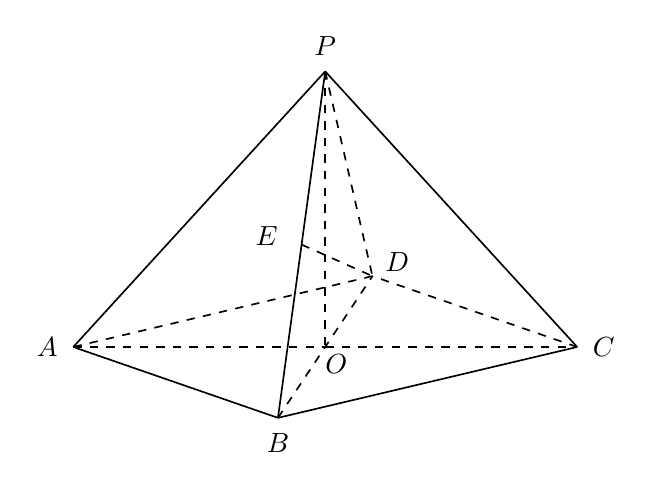
\begin{tikzpicture}[x=1cm,y=1cm,font=\normalsize,line width=.6pt]
\coordinate (P) at (0.0000000000,3.5000000000);
\coordinate (A) at (-3.2,0);
\coordinate (C) at (3.2,0);
\coordinate (O) at (0,0);
\coordinate (B) at (-0.6,-0.9);
\coordinate (D) at (0.6000000000,0.9000000000);
\coordinate (E) at (-0.3000000000,1.3000000000);
% lateral edges
\draw[solid] (P) -- (A);
\draw[solid] (P) -- (B);
\draw[solid] (P) -- (C);
\draw[dashed] (P) -- (D);
\draw[dashed] (P) -- (O);
\draw[dashed] (E) -- (D);
% base perimeter
\draw[solid] (A) -- (B);
\draw[solid] (B) -- (C);
\draw[dashed] (C) -- (D);
\draw[dashed] (D) -- (A);
% base diagonals through O
\draw[dashed] (A) -- (O);
\draw[dashed] (O) -- (C);
\draw[dashed] (B) -- (D);
% labels
\node[above=2pt] at (P) {$P$};
\node[left=2pt] at (A) {$A$};
\node[below=2pt] at (B) {$B$};
\node[right=2pt] at (C) {$C$};
\node[right=2pt,xshift=-1pt,yshift=5pt] at (D) {$D$};
\node[below=3pt,xshift=4pt,yshift=4pt] at (O) {$O$};
\node[left=2pt,xshift=-3pt,yshift=3pt] at (E) {$E$};
\end{tikzpicture}
